\documentclass[12pt]{article}
\usepackage{amsmath}
\usepackage{booktabs}
\usepackage{graphicx}

\newcommand{\brak}[1]{\left( #1 \right)} 

\title{Discrete Assignment-11.9.1-11}
\author{Hiba Muhammed \\
        EE23BTECH11026}
\date{} 

\begin{document}

\maketitle

\section*{Problem Statement}
Write the first five terms in the sequence:
\begin{align}
a_{0}  &= 3 \\
a_{n}  &= 3a_{n-1} + 2 \quad \text{for } n > 0
\end{align}

\section*{Solution}

\begin{table}[h]
  \centering
  \caption{Input Parameters: First Term and General Formula}
  \begin{tabular}{|c|c|}
    \hline
    \textbf{Term} & \textbf{Value} \\
    \hline
    $\brak{x(0)}$ & 3 \\
    $\brak{x(n)}$ & $\brak{3x(n-1) + 2}$ for $n > 0$ \\
    \hline
  \end{tabular}
\end{table}

So, the first 5 terms of the sequence are $\brak{3, 11, 35, 107, 323}$.


\subsection*{Difference Equation and Z-transform}

The given difference equation is:
\begin{align}
y(n) &= 3y(n-1)x(n-1) - x(n-1) + 3x(n) \\
x(n) &= u(n) \\
y(n) &= 3y(n-1)u(n-1) - u(n-1) + 3u(n)
\end{align}

\textbf{Parameter}

Z-transform of the difference equation is:
\begin{align}
Y(z) &= \frac{3z^{-1}Y(z) - z^{-1} + 3}{1 - z^{-1}}
\end{align}

\begin{align}
Y(z) &= \frac{2(1 - z^{-1})}{z^{-2} - 2z^{-1} - 2}
\end{align}

\begin{figure}[h]
    \centering
    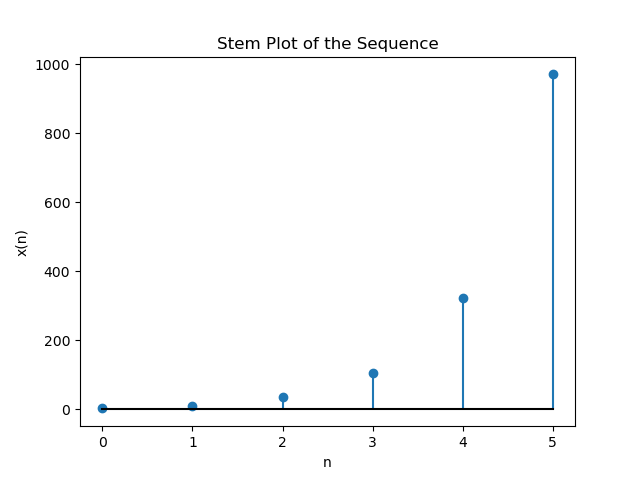
\includegraphics[width=0.8\textwidth]{11.9.1-11.png}
    \caption{Sequence}
\end{figure}

\end{document}

